\chapter{Computational Methods} \label{ch:3}

\section{The Particle-In-Cell Method}

The Particle-In-Cell (PIC) method involves solving Maxwell's Equations on a grid 

\begin{align}
	\nabla \cdot \vec{E} &= \frac{\rho}{\epsilon_0}  \label{eq:gauss} \\
	\nabla \times \vec{E} &= - \frac{\partial \vec{B}}{\partial t} \label{eq:faraday} \\
	\nabla \cdot \vec{B} &= 0 \label{eq:gauss_magnetism} \\
	\nabla \times \vec{B} &= \mu_0 (\vec{J} + \epsilon_0 \frac{\partial \vec{E}}{\partial t}) \label{eq:ampere}
\end{align}
This is combined with the lorentz force

\begin{equation}
	\vec{F} = q(\vec{E} + \vec{v} \times \vec{B}) \label{eq:lorentz_pic}
\end{equation}
which determines the motions (i.e. $\vec{r}$ and $\vec{v}$) of charged particles by integration. It is impossible to keep track of the true numbers of particles in this type of simulation which would be roughly on the order of Avogadro's number $\sim 10^{23}$. Instead, we lump many particles together into what is called a \emph{macro particle}. For example, one ``macro electron'' could contain 1 trillion ``real electrons''. Also, we cannot hope to have infinite precision in calculating quantities of interest. Spatially, we must separate the simulation volume into a grid where each cell has length $\Delta x$, $\Delta y$, and $\Delta z$ in the x, y, and z direction respectively. Temporally, we introduce a time step $\Delta t$ which allows us to propagate Maxwell's Equations forward in time by $\Delta t$ for every iteration.

For simplicity, non-relativistic equations will be introduced in this section, but they can easily be generalized to the relativistic versions which are implemented in modern PIC codes. Additionally, some of the equations will assume a 2D grid, but a 3D grid is similarly straightforward to generalize.

\subsection{Densities and Shape Factors}

When a simulation is initialized, all the particles will have a defined position and velocity. The charge density $\rho_{i,j}$ (for the cell at the $i^\text{th}$ and $j^\text{th}$ grid point in the x and y directions) is easy to compute -- it is simply the sum of all the charges $q_\alpha$ closest to grid point $(i,j)$ divided by the cell area: $\rho_{i,j} \equiv \frac{\sum_\alpha q_\alpha}{\Delta x \Delta y}$ (in 2D symmetry we additionally divide by 1 meter in the z direction to get the units right). The current density $\vec{J}_{i,j}$ can be obtained similarly -- $\vec{J}_{i,j} \equiv \frac{\sum_\alpha q_\alpha \vec{v}_\alpha}{\Delta x \Delta y}$. Assigning the densities to the nearest grid point in this manner is sensibly called Nearest Grid Point (NGP) by Birdsall and Langdon \cite{Birdsall_2004_PIC}.

Since the PIC approach contains many real particles in each macro particle, it is desired to smooth the macro particle densities throughout the cell(s). We can modify the individual density contributions of particles by a shape factor $S(\vec{r_\alpha} - \vec{r})$ that depends on a particle's location $\vec{r_\alpha}$ in relation to a grid point located at $\vec{r}$. This shape factor is normalized so that integrating it over the area of the simulation yields 1 to ensure the particle number is properly being conserved. The simplest improvement over NGP would be the \emph{top hat} shape factor (also called Cloud in Cell \cite{Birdsall_2004_PIC}) which assigns density contributions proportional to proximity of the nearest cells within ($\Delta x$,$\Delta y$). This has the shape of a uniform distribution and thus looks like a ``top hat'' in 1D. It is a $0^\text{th}$ order shape factor and can be represented by the following equation

\begin{equation}
	S_0(x) \equiv \begin{cases}
		1 & \text{if } \lvert x \rvert \leq 0.5 \Delta x \\
		0 & \text{otherwise}
	\end{cases} \label{eq:tophat}
\end{equation}
A further improvement will weigh the particles closer to a particular grid point higher than a particle further away. If this weighting is linear over an area ($2 \Delta x$, $2 \Delta y$), it is called the \emph{triangle} shape factor and reprsented by the following equation in 1D

\begin{equation}
	S_1(x) \equiv \begin{cases}
		1-\frac{\lvert x \rvert}{\Delta x} & \text{if } \lvert x \rvert \leq \Delta x \\
		0 & \text{otherwise}
	\end{cases} \label{eq:triangle}
\end{equation}
It turns out that the higher order shape factors $S_n(x)$ can be represented by convolutions of $S_0(x)$ 

\begin{figure}
	\centering 
	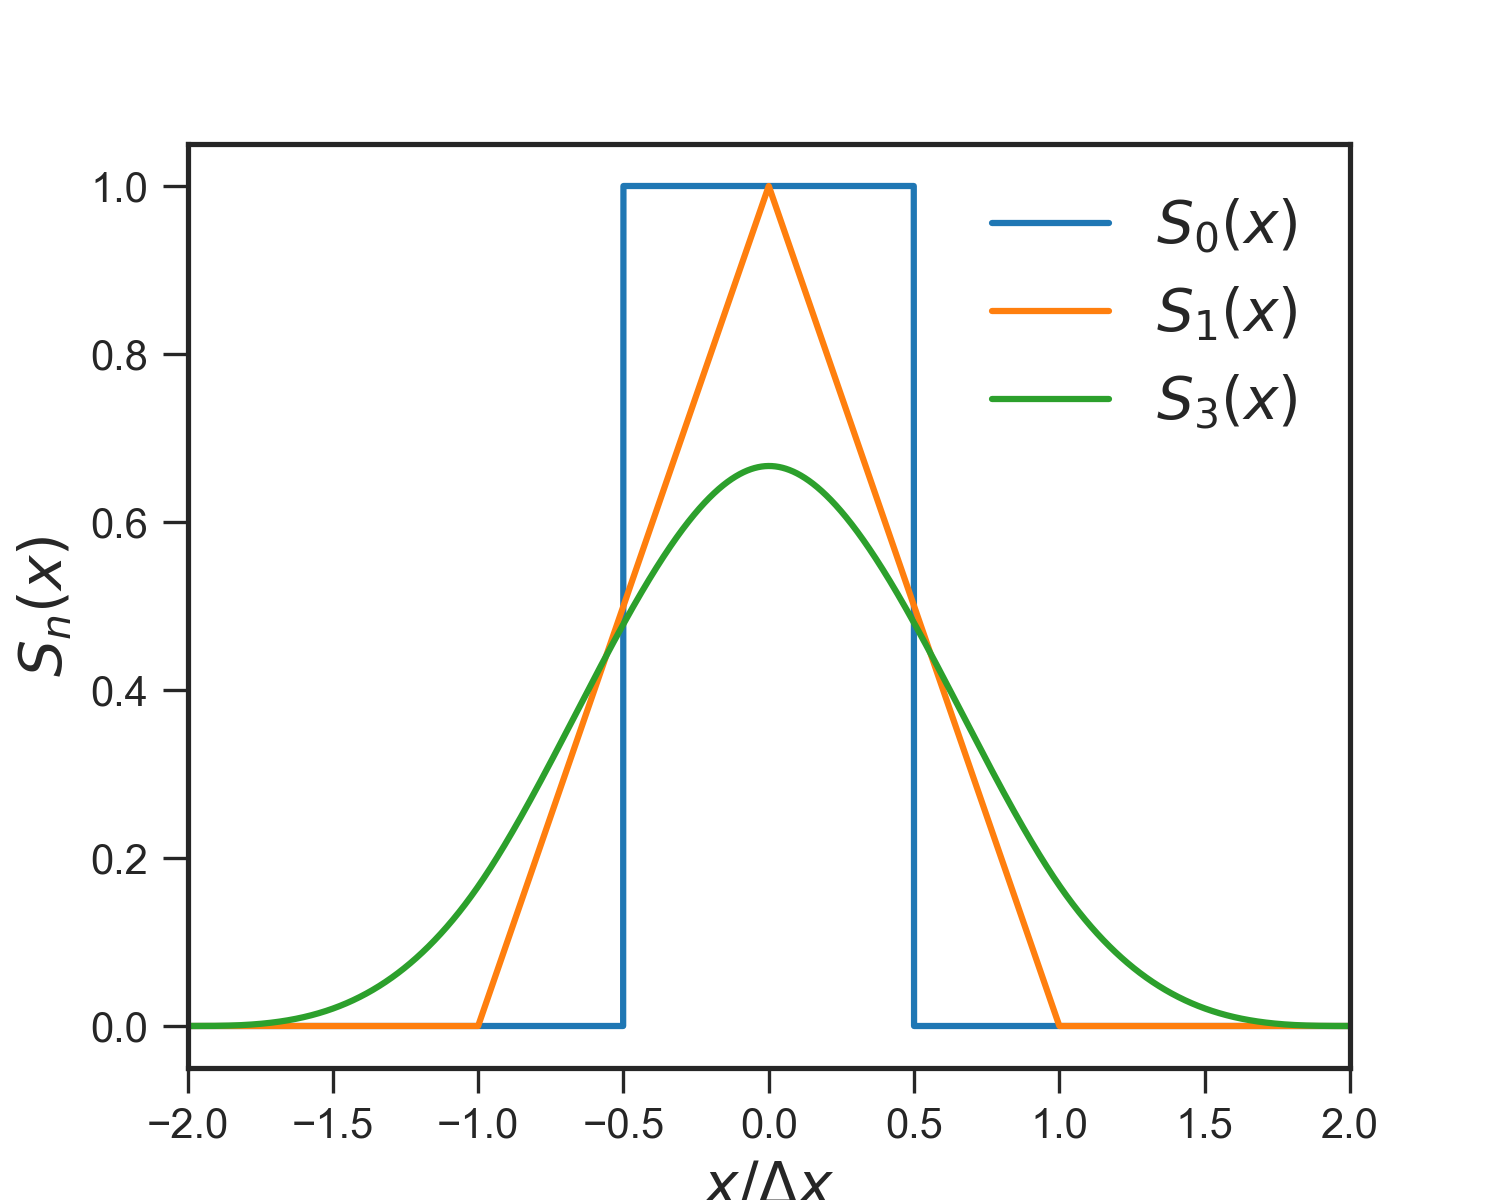
\includegraphics[width=0.6\linewidth]{planning/images/shape_functions.png}
	\caption{The top hat ($S_0(x)$), triangle ($S_1(x)$) and $3^\text{rd}$ order spline ($S_3(x)$) are plotted in 1D.}
	\label{fig:shape_factors}
\end{figure}

\begin{equation}
	S_n(x) \equiv \int_{-\infty}^\infty S_{n-1}(x')S_0(x-x') dx'
\end{equation}
and the shape factors for $n \geq 2$ are commonly called n-splines. The third order spline is used in this work and weights particles over an area ($4 \Delta x$, $4 \Delta y$) and is represented in 1D by 

\begin{equation}
	b_3(x) = \begin{cases}
		\frac{1}{6}(8 - 12 \lvert \tilde{x} \rvert + 6 \tilde{x}^2 - \tilde{x}^3) & \text{if } 1 \leq \lvert \tilde{x} \rvert \leq 2 \\
		\frac{1}{6}(4 - 6 \tilde{x}^2 + 3 \tilde{x}^3) & \text{if } \lvert \tilde{x} \rvert \leq 1 \\
		0 & \text{otherwise}
	\end{cases}
\end{equation}
where $\tilde{x} \equiv x / \Delta x$ normalizes the position $x$. See \cref{fig:shape_factors} for a comparison of the three shape factors. 

These shape factors not only apply to the calculation of densities, but also to the electric and magnetic fields. In this way, the fields used to update particle positions and velocities are averaged over neighboring cells.

\subsection{Field Solver and Particle Push}

\begin{figure}
	\centering 
	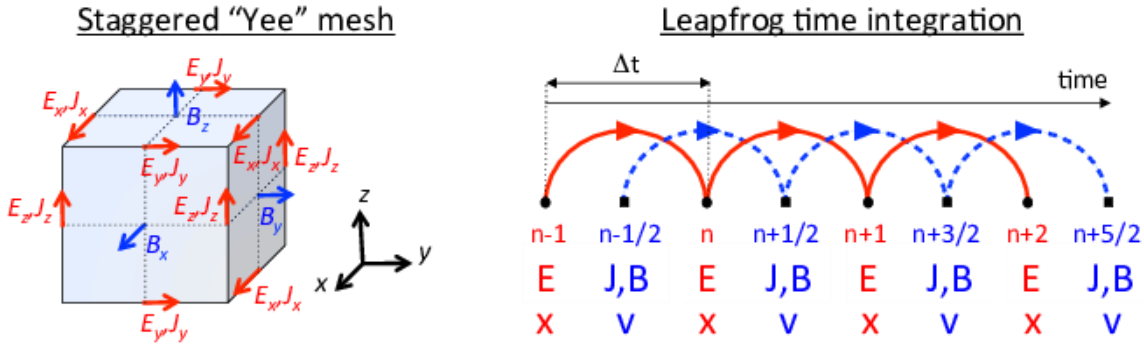
\includegraphics[width=0.8\linewidth]{planning/images/yee_grid.PNG}
	\caption{The ``Yee'' grid is depicted (left) where the electric and magnetic field components are staggered by half a cell. The fields, currents, position, and velocity make use of the staggered grid by leapfrog time integration (right). This picture was taken from the WarpX documentation}
	\label{fig:yee_grid}
\end{figure}

The PIC method is able to make efficient use of the second order accurate central difference approximation to compute derivatives. A simpler method like Euler integration is only first order accurate and will suffer in terms of accuracy. Higher order methods like 4th order Runge-Kutta have much higher computational costs in terms of operations per time step and memory consumption. The central difference scheme is accomplished by alternately calculating electric and magnetic fields, staggered by half a time step, in an approach called \emph{leapfrog integration} \cite{Birdsall_2004_PIC}. This can be seen in the right half of \cref{fig:yee_grid} where the calculations of $E$ and $J,B$ alternate in a ``leapfrog'' fashion. It turns out that this staggering also comes with some nice properties like automatically satisfying \cref{eq:gauss_magnetism}. By rearranging \cref{eq:faraday}, we can update the electric and magnetic fields through the following equations \cite{Arber_2015_PPCF}

\begin{align}
	\vec{E}^{n+1} &= \vec{E}^{n} + \Delta t (c^2 \nabla \times \vec{B}^{n+\frac{1}{2}} - \frac{1}{\epsilon_0} \vec{J}^{n+\frac{1}{2}}) \label{eq:E_update} \\
	\vec{B}^{n+\frac{1}{2}} &= \vec{B}^{n-\frac{1}{2}} - \Delta t (\nabla \times \vec{E}^{n}) \label{eq:B_update}
\end{align}
where $\vec{J}^{n+\frac{1}{2}} \equiv \frac{\sum_\alpha q_\alpha \vec{v}^{n+\frac{1}{2}}_\alpha}{\Delta x \Delta y}$ depends on the velocity. The updated velocity for each particle is calculated through the force from \cref{eq:lorentz_pic}. 

\begin{equation}
	\frac{v^{n + \frac{1}{2}}_\alpha - v^{n - \frac{1}{2}}_\alpha}{\Delta t} = \frac{q}{m}[E^n_\alpha + \frac{v^{n + \frac{1}{2}}_\alpha + v^{n + \frac{1}{2}}_\alpha}{2} \times B^n_\alpha] \label{eq:v_update}
\end{equation}
The $\alpha$ subscript indicates the quantities are calculated for each particle; thus, the fields are smoothed out by the shape factor (e.g. $E^n_\alpha \equiv \int E^n S_3(x-x_\alpha, y-y_\alpha, z-z_\alpha) dx \; dy \; dz$). In practice, \cref{eq:B_update,eq:E_update} are broken up into half-steps so that the electric and magnetic field are known for all half-steps. At first glance, \cref{eq:v_update} does not appear to have an explicit solution for $v^{n + \frac{1}{2}}$. There are implicit methods that can solve this equation which are used in codes like LSP \cite{Welch_2004_LSP}. It turns out that there is an explicit solution given by the \emph{Boris Rotation Algorithm}. If we define 

\begin{align}
	v^{n + \frac{1}{2}} &= v^+ + \frac{q E^n}{2 m} \Delta t \label{eq:vplus} \\
	v^{n - \frac{1}{2}} &= v^- - \frac{q E^n}{2 m} \Delta t \label{eq:vminus}
\end{align}
we can separate out the electric field dependence to get 

\begin{equation}
	\frac{v^+ - v^-}{\Delta t} = \frac{q}{m}[\frac{v^+ + v^-}{2} \times B]
\end{equation}
which can conveniently be calculated through a rotation \cite{Birdsall_2004_PIC} through the following steps:

\begin{enumerate}
	\item Compute $v^-$ from \cref{eq:vminus}.
	\item Compute $\vec{t} \equiv \frac{q \Delta t}{2 m} \vec{B}^n $ (equivalent in magnitude to $\tan(\theta/2)$ where $\theta$ is the rotation angle)
	\item Compute $\vec{s} = \frac{2 \vec{t}}{1 + t^2}$ (equivalent in magnitude to $\sin(\theta/2)$)
	\item Compute $\vec{v}' = \vec{v}^- + \vec{v}^- \times \vec{t}$.
	\item Compute $\vec{v}^{n+\frac{1}{2}}$ from \cref{eq:vplus}.
\end{enumerate}
Now, the particles can be advanced or ``pushed'' from

\begin{equation}
	x^{n+1} = x^{n} + v^{n+\frac{1}{2}} \Delta t \label{eq:particlepush}
\end{equation}
For completeness, the velocity initially needs to be pushed backwards from $v^{0} \rightarrow v^{-\frac{1}{2}}$. This is not done in a time-centered way, but is only needed at the start of the simulation. 

\subsection{EPOCH Code}

\begin{quote}
	Clearly Top-hat shape functions should never be used for laser-solid simulations.
\end{quote}

\subsubsection{Background}

\subsubsection{Methods}

\subsubsection{Results}

\section{Machine Learning}

\subsection{Simple Models}

\subsubsection{Polynomial Regression}

\subsubsection{Support Vector Regression}


\subsection{Advanced Models}

\subsubsection{Gaussian Process}

\subsection{Neural Networks}